%!TEX program = xelatex
%%%%%%%%%%%%%%%%%%%%%%%这是导言部分的开始%%%%%%%%

%========= 导言部分声明文档的类型=================
\documentclass{article}

	%=========导言部分可可以加载宏包=================
	\usepackage{amsmath}                % 数学公式排版宏包
	\usepackage{amssymb}                % 数学符号命令宏包
	\usepackage{amsthm}                 % 数学定理宏包
	\usepackage[UTF8]{ctex}             % 中文输入宏包
	\usepackage[a4paper]{geometry}      % 页面设置宏包
	\usepackage{setspace}               % 行间距宏包
	\usepackage{graphicx}               % 图片宏包
	\usepackage{listings}               % 代码宏包
	\usepackage{color}					% 颜色宏包
	\usepackage{xcolor}                 % 颜色处理宏包
	\usepackage{float}                  % 浮动对象式样宏包
	\usepackage{fontspec}
	\usepackage{enumerate}				% 列举编号包
	
	%=========页面设置==============================
	\geometry{left=1cm,right=1cm,top=1cm,bottom=2cm}
	\onehalfspacing
	\setlength\parindent{0em}

	%=========代码格式设置============================
	\definecolor{dkgreen}{rgb}{0,0.6,0}
	\definecolor{gray}{rgb}{0.5,0.5,0.5}
	\definecolor{mauve}{rgb}{0.58,0,0.82}
	% \setmonofont{Consolas}
	\lstset{
		numbers = left, 	
		numberstyle = \color{gray}, 
		keywordstyle = \color{blue},
		commentstyle = \color{dkgreen}, 
		stringstyle = \color{mauve},
		basicstyle = \ttfamily,
		breaklines = true,
		frame = shadowbox, % 阴影效果
		rulesepcolor = \color{ red!20!green!20!blue!20} ,
		escapeinside = ``, % 英文分号中可写入中文
		xleftmargin = 2em,xrightmargin=2em, aboveskip=1em,
		framexleftmargin = 2em
	} 

%=========导言部分可以定义标题信息===============
\title{组会报告}
\author{徐益}
\date{\today}
%%%%%%%%%%%%%%%%%%%%%%%这是导言部分的结束%%%%%%%%%

%%%%%%%%%%%%%%%%%%%%%%%这是正文部分的开始%%%%%%%%%
\begin{document}

%=========生成标题================================
\maketitle

%=========开始正文的输入==========================

%===========第一节=================
\section{工作内容}
1. 实现与原fixed-layered-OMS误码一致的avx2-OMS译码模块,并测试吞吐量。

2. 尝试提高吞吐量。

3. 尝试解决fixed-OMS译码曲线出现的“平台”现象。

%===========第一节=================
\section{实现avx2-OMS译码模块}
\begin{table}[H]
	\caption{不同译码算法的吞吐量($SNR=1.6dB(BER<10^{-5}), N=25344,R=0.5,I_{max}=10$)}
	\centering
	\begin{tabular}{|l|l|l|l|l|}% 通过添加 | 来表示是否需要绘制竖线
		\hline  % 在表格最上方绘制横线
		scheduling	& BP		& float-OMS	&	fixed-OMS	& avx2-OMS	\\
		\hline
		Throuput	& 0.190Mbps	& 0.572Mbps	&	0.4160Mbps	& 6.744Mbps	\\
		\hline  % 在表格最下方绘制横线
	\end{tabular}
\end{table}

%===========第二节=================
\section{尝试提高吞吐量}
加入判决机制:
\begin{table}[H]
	\caption{不同译码算法的吞吐量($SNR=1.6dB(BER<10^{-5}), N=25344,R=0.5,I_{max}=10$)}
	\centering
	\begin{tabular}{|l|l|l|l|l|}% 通过添加 | 来表示是否需要绘制竖线
		\hline  % 在表格最上方绘制横线
		scheduling	&	avx2-OMS	& avx2-OMS with judgment	\\
		\hline
		Throuput	&	6.744Mbps	& 5.573Mbps					\\
		\hline  % 在表格最下方绘制横线
	\end{tabular}
\end{table}

%===========第三节=================
\section{尝试解决fixed-OMS译码曲线出现的“平台”现象}
\subsection{消除float转int8\_t时inf造成的影响}
原方案:
\lstset{language=C++}
\begin{lstlisting}
for (i = 0; i < Nd; i++)
{
	temp_llr = (int32_t)llr[i] * FACTOR_BETA;
	if (temp_llr > MAX_FIXED_MSG)
		llr_fixed[i] = MAX_FIXED_MSG;
	else if (temp_llr < MIN_FIXED_MSG)
		llr_fixed[i] = MIN_FIXED_MSG;
	else
		llr_fixed[i] = (int8_t)(llr[i]*FACTOR_BETA);
}
\end{lstlisting}
现方案:
\lstset{language=C++}
\begin{lstlisting}
for (i = 0; i < Nd; i++)
{
	if (llr[i] >= 4)
		llr_fixed[i] = MAX_FIXED_MSG;
	else if (llr[i] <= -4)
		llr_fixed[i] = MIN_FIXED_MSG;
	else
		llr_fixed[i] = (int8_t)(llr[i]*FACTOR_BETA);
}
\end{lstlisting}
\subsection{使饱和后的cn\_msg保持不变}
原方案:
\lstset{language=C++}
\begin{lstlisting}
omin_llr = VECTOR_MAX(VECTOR_SUB(min_llr, vbeta), VECTOR_ZERO);
osubmin_llr = VECTOR_MAX(VECTOR_SUB(submin_llr, vbeta), VECTOR_ZERO);
\end{lstlisting}
现方案:
\lstset{language=C++}
\begin{lstlisting}
min_temp = VECTOR_MAX(VECTOR_SUB(min_llr, vbeta), VECTOR_ZERO);
submin_temp = VECTOR_MAX(VECTOR_SUB(submin_llr, vbeta), VECTOR_ZERO);
/* if(min_llr==max_msg) omin_llr=vmax_msg; else omin_llr=min_temp */
omin_llr = VECTOR_CMOV(min_llr, vmax_msg, vmax_msg, min_temp);
osubmin_llr = VECTOR_CMOV(submin_llr, vmax_msg, vmax_msg, submin_temp);
\end{lstlisting}
\subsection{误码性能对比}
\begin{figure}[H]
	\centering
	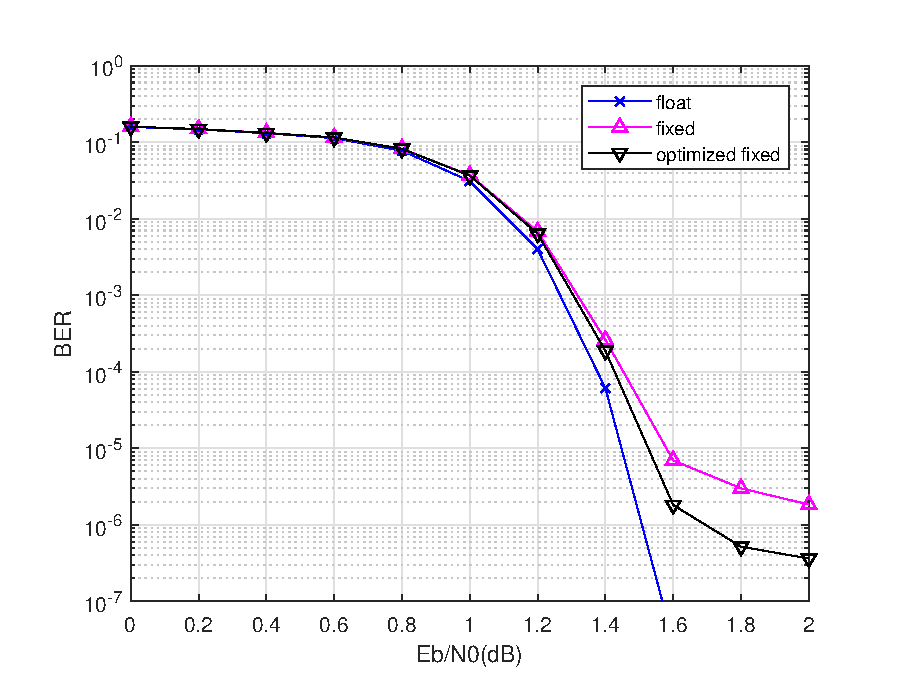
\includegraphics[width = .7\textwidth]{fig.eps}
	\caption{优化前后误码性能对比($N=25344,R=0.5,I_{max}=10$)}
\end{figure}
\subsection{吞吐量对比}
\begin{table}[H]
	\caption{不同译码算法的吞吐量($SNR=1.6dB(BER<10^{-5}), N=25344,R=0.5,I_{max}=10$)}
	\centering
	\begin{tabular}{|l|l|l|l|l|}% 通过添加 | 来表示是否需要绘制竖线
		\hline  % 在表格最上方绘制横线
		scheduling	&	avx2-OMS	& optimized avx2-OMS	\\
		\hline
		Throuput	&	6.744Mbps	& 6.689Mbps				\\
		\hline  % 在表格最下方绘制横线
	\end{tabular}
\end{table}

%===========第四节=================
% \section{仍存在问题}


%===========下周计划=================
\section{下阶段计划}
1. 进一步优化avx2-oms算法

2. 尝试avx2-nms算法的实现

\end{document}
%%%%%%%%%%%%%%%%%%%%%%%这是正文部分的结束%%%%%%%%%%%%